\documentclass[12pt,a4paper]{article}
% math_setup.tex
% Essential Packages
\RequirePackage{etex}
\usepackage{comment}
\usepackage{etex}
\usepackage{listings}
\usepackage{amsmath}    % Advanced math typesetting
\usepackage{amsfonts}   % Math fonts
\usepackage{amssymb}    % Math symbols
\usepackage{amsthm}     % Theorem environment
\usepackage{mathtools}  % More symbols
\usepackage{tikz}       % For drawing diagrams
\usepackage{tikz-network}
\usepackage{pgfplots}
\usetikzlibrary{calc, arrows.meta, positioning, quotes}
\usepackage{mdframed}
\usepackage{float}
\usepackage{thmtools}
\usepackage{xcolor}
\usepackage{geometry}
\usepackage{fancyhdr}
\usepackage[colorlinks=true, linkcolor=blue, citecolor=green, urlcolor=red]{hyperref}
\usepackage{csquotes}
\usepackage[backend=biber, style=ieee]{biblatex}
\pgfplotsset{compat=1.18}
%\usepackage{mdframed}

% Wolfram Code Block
\lstdefinelanguage{Wolfram}{
    keywords={Sum, If, For, While, Do, Plot, Table, Range, Integrate, NIntegrate, D, Solve, NSolve, DSolve, NDSolve, LinearSolve, Expand, Factor, Simplify, FullSimplify, Module, Block, With},
    sensitive=true,
    morecomment=[l]{(*},
    morecomment=[s][\itshape]{(*}{*)},
    morestring=[b]",
    morestring=[b]',
}

\lstset{
    language=Wolfram,
    basicstyle=\ttfamily,
    keywordstyle=\color{blue}\bfseries,
    commentstyle=\color{green}\itshape,
    stringstyle=\color{red},
    showstringspaces=false,
    frame=single,
    breaklines=true,
    numbers=left,
    numberstyle=\tiny\color{gray},
    stepnumber=1,
    numbersep=5pt,
    backgroundcolor=\color{lightgray!20}
}

% add ref
\addbibresource{references.bib}
% Define colors
\definecolor{theoremcolor}{RGB}{230,230,250}  % Light purple
\definecolor{lemmacolor}{RGB}{240,248,255}    % Alice Blue
\definecolor{propcolor}{RGB}{240,255,240}     % Light green
\definecolor{corollarycolor}{RGB}{255,250,240} % Light orange
\definecolor{axiomcolor}{RGB}{255,240,245}    % Lavender blush
\definecolor{definitioncolor}{RGB}{240,255,255} % Light cyan
\definecolor{remarkcolor}{RGB}{245,245,245}   % Light gray
\definecolor{notationcolor}{RGB}{255,250,205}

% Boxed environments

\declaretheoremstyle[
    headfont=\normalfont\bfseries,
    bodyfont=\normalfont,
    headpunct={:},
    postheadspace=1em,
    mdframed={
        linecolor=black,
        backgroundcolor=definitioncolor,
        topline=true,
        bottomline=true,
        leftline=true,
        rightline=true,
        roundcorner=5pt
    }
]{boxeddefinitionstyle}

\declaretheorem[style=boxeddefinitionstyle, name=Definition]{definition}

\declaretheoremstyle[
    headfont=\normalfont\bfseries,
    bodyfont=\normalfont,
    headpunct={:},
    postheadspace=1em,
    mdframed={
        linecolor=black,
        backgroundcolor=theoremcolor,
        topline=true,
        bottomline=true,
        leftline=true,
        rightline=true,
        roundcorner=5pt
    }
]{boxedtheoremstyle}

% Theorem
\declaretheorem[style=boxedtheoremstyle, name=Theorem]{theorem}

% Lemma (adjust color)
\declaretheoremstyle[
    headfont=\normalfont\bfseries,
    bodyfont=\normalfont,
    headpunct={:},
    postheadspace=1em,
    mdframed={
        linecolor=black,
        backgroundcolor=lemmacolor,
        topline=true,
        bottomline=true,
        leftline=true,
        rightline=true,
        roundcorner=5pt
    }
]{boxedlemmastyle}
\declaretheorem[style=boxedlemmastyle, name=Lemma]{lemma}

% Proposition (adjust color)
\declaretheoremstyle[
    headfont=\normalfont\bfseries,
    bodyfont=\normalfont,
    headpunct={:},
    postheadspace=1em,
    mdframed={
        linecolor=black,
        backgroundcolor=propcolor,
        topline=true,
        bottomline=true,
        leftline=true,
        rightline=true,
        roundcorner=5pt
    }
]{boxedpropstyle}
\declaretheorem[style=boxedpropstyle, name=Proposition]{proposition}

% Corollary (adjust color)
\declaretheoremstyle[
    headfont=\normalfont\bfseries,
    bodyfont=\normalfont,
    headpunct={:},
    postheadspace=1em,
    mdframed={
        linecolor=black,
        backgroundcolor=corollarycolor,
        topline=true,
        bottomline=true,
        leftline=true,
        rightline=true,
        roundcorner=5pt
    }
]{boxedcorollarystyle}
\declaretheorem[style=boxedcorollarystyle, name=Corollary]{corollary}

% Axiom (boxed)
\declaretheoremstyle[
    headfont=\normalfont\bfseries,
    bodyfont=\normalfont,
    headpunct={:},
    postheadspace=1em,
    mdframed={
        linecolor=black,
        backgroundcolor=axiomcolor,
        topline=true,
        bottomline=true,
        leftline=true,
        rightline=true,
        roundcorner=5pt
    }
]{boxedaxiomstyle}
\declaretheorem[style=boxedaxiomstyle, name=Axiom]{axiom}

% Remark environment
\declaretheoremstyle[
    headfont=\normalfont\bfseries,
    bodyfont=\normalfont,
    headpunct={:},
    postheadspace=1em,
    mdframed={
        linecolor=black,
        backgroundcolor=remarkcolor,
        topline=true,
        bottomline=true,
        leftline=true,
        rightline=true,
        roundcorner=5pt
    }
]{remarkstyle}
\declaretheorem[style=remarkstyle, name=Remark, numbered=no]{remark}
% Normal, non-italic environments
\declaretheoremstyle[
    headfont=\normalfont\bfseries,
    bodyfont=\normalfont,
    headpunct={:},
    postheadspace=1em,
]{normalstyle}

% Notation environment
\declaretheoremstyle[
    headfont=\normalfont\bfseries,
    bodyfont=\normalfont,
    headpunct={:},
    postheadspace=1em,
    mdframed={
        linecolor=black,
        backgroundcolor=notationcolor,
        topline=true,
        bottomline=true,
        leftline=true,
        rightline=true,
        roundcorner=5pt
    }
]{boxednotationstyle}
\declaretheorem[style=boxednotationstyle, name=Notation]{notation}


% Note environment (more noticeable, with separators, no background, no end symbol)
\newenvironment{note}[1][]
    {\par\vspace{0.5em}\noindent\rule{\textwidth}{0.4pt}\par\vspace{0.5em}%
    \textbf{Note\if\relax\detokenize{#1}\relax\else: #1\fi}\par}
    {\par\vspace{0.5em}\noindent\rule{\textwidth}{0.4pt}\par\vspace{0.5em}}

\declaretheorem[style=normalstyle, name=Note, numbered=no]{oldnote}

\declaretheorem[style=normalstyle, name=Example]{example}
\declaretheorem[style=normalstyle, name=Exercise]{exercise}
\declaretheorem[style=normalstyle, name=Statement]{statement}
\declaretheorem[style=normalstyle, name=Solution, numbered=no]{solution}

% Proof environment (normal, non-italic, with QED symbol)
\declaretheoremstyle[
    headfont=\normalfont\bfseries,
    bodyfont=\normalfont,
    headpunct={:},
    postheadspace=1em,
    qed=$\blacksquare$
]{proofstyle}

\declaretheorem[style=proofstyle, name=Proof]{customproof}

% Shorthand
\newcommand{\vect}[1]{\mathbf{#1}} % For regular vectors
\newcommand{\uvec}[1]{\hat{\mathbf{#1}}} % For unit vectors
\newcommand{\prob}[1]{
    \section*{Problem #1}
}
\newcommand{\R}{\mathbb{R}} % Real numbers
\newcommand{\Z}{\mathbb{Z}} % Integers
\newcommand{\C}{\mathbb{C}} % Complex numbers
\newcommand{\N}{\mathbb{N}} % Natural numbers
\newcommand{\Q}{\mathbb{Q}} % Rational numbers
\newcommand{\Hq}{\mathbb{H}} % Quaternions
\newcommand{\F}{\mathbb{F}} % Finite fields
\newcommand{\Proj}{\mathbb{P}} % Projective space
\newcommand{\K}{\mathbb{K}} % Arbitrary field
\newcommand{\T}{\mathbb{T}} % Torus or sometimes denoted for Topological space
\newcommand{\A}{\mathbb{A}} % Affine space
\newcommand{\0}{\mathbf{0}} % Zero vector
\newcommand{\mbf}[1]{\mathbf{#1}} 
\newcommand{\mat}[1]{\mathbf{#1}}
\newcommand{\adj}{\operatorname{adj}}
\newcommand{\dom}[1]{
    \operatorname{dom}(#1)
}




% Layout
\geometry{a4paper, margin=1in}
\pagestyle{fancy}
\fancyhf{}
\rhead{\today}
\lhead{\textbf{ENG1005 Engineering Mathematics}}
\rfoot{Page \thepage}


\newcommand{\drawV}[3]{
    \Vertex[x=#1, y=#2, size = 1, label = $#3$, fontscale = 1.5]{#3}
}

\newcommand{\drawL}[4]{
    \Edge[loopposition=#1, loopshape=#2, Direct, label = #3, fontscale = 1.2](#4)(#4)
}

\newcommand{\drawE}[4][0]{
    \Edge[Direct, bend = #1, label = #2, fontscale = 1.2](#3)(#4)
}

\newcommand{\num}[1]{
    \operatorname{num}(#1)
}

\begin{document}
\title{ENG1005 Week4 Workshop Problem Set Solutions}
\author{Yang Xingyu (33533563)}
\date{\today}
\maketitle


\section*{Applied Class Challenge}
\begin{theorem}[Eigenvalues of Triangular Matrices]
    Let \( A \) be an \( n \times n \) upper or lower triangular matrix. Then the eigenvalues of \( A \) are precisely the entries on the diagonal of \( A \). That is, the eigenvalues of \( A \) are \( \lambda_1 = a_{11}, \lambda_2 = a_{22}, \dots, \lambda_n = a_{nn} \).
\end{theorem}

\begin{proof}[Inductive Proof]
We will prove the theorem by induction. Let the predicate \( P(n) \) denote that for an \( n \times n \) matrix \( \mathbf{A} \), the eigenvalue \( \lambda_n = a_{nn} \), where \( n \in \mathbb{Z}_{\geq 1} \).

\textbf{Base Case:}  
When \( n = 1 \), we have \( |\mathbf{A} - \lambda \mathbf{I}| = 0 \implies a_{11} - \lambda_1 = 0 \). Hence, \( a_{11} = \lambda_1 \), so \( P(1) \) holds.

\textbf{Inductive Step:}  
Assume that \( P(n) \) holds as stated in the theorem. We will now prove that \( P(n+1) \) also holds.

Suppose we have the matrix
\[
A = \begin{bmatrix}
a_{11} & a_{12} & \cdots & a_{1n} \\
0 & a_{22} & \cdots & a_{2n} \\
\vdots & \vdots & \ddots & \vdots \\
0 & 0 & \cdots & a_{nn}
\end{bmatrix},
\]
and
\[
B = \begin{bmatrix}
a_{11} & a_{12} & \cdots & a_{1n} & a_{1,n+1} \\
0 & a_{22} & \cdots & a_{2n} & a_{2,n+1} \\
\vdots & \vdots & \ddots & \vdots & \vdots \\
0 & 0 & \cdots & a_{nn} & a_{n,n+1} \\
0 & 0 & \cdots & 0 & a_{n+1,n+1}
\end{bmatrix}.
\]
where \( \mathbf{B} \) is obtained from the matrix \( \mathbf{A} \) by adding some random real or complex entries in the last column.

To find the eigenvalues, we need to solve \( \mathbf{B} - \lambda \mathbf{I} = \mathbf{0} \). 
\[
|\mathbf{B} - \lambda \mathbf{I}| = \begin{vmatrix}
a_{11} - \lambda & a_{12} & \cdots & a_{1n} & a_{1,n+1} \\
0 & a_{22} - \lambda & \cdots & a_{2n} & a_{2,n+1} \\
\vdots & \vdots & \ddots & \vdots & \vdots \\
0 & 0 & \cdots & a_{nn} - \lambda & a_{n,n+1} \\
0 & 0 & \cdots & 0 & a_{n+1,n+1} - \lambda
\end{vmatrix} = 0
\]
Now, we extract the common factors of the determinant by row and column, respectively, as shown below.

\begin{align*}
|\mathbf{B -\lambda \mathbf{I}}| &= \begin{vmatrix}
a_{11} - \lambda & a_{12} & \cdots & a_{1n} & a_{1,n+1} \\
0 & a_{22}-\lambda & \cdots & a_{2n} & a_{2,n+1} \\
\vdots & \vdots & \ddots & \vdots & \vdots \\
0 & 0 & \cdots & a_{nn} -\lambda & a_{n,n+1} \\
0 & 0 & \cdots & 0 & a_{n+1,n+1} -\lambda
\end{vmatrix} =0\\
&= (a_{11} - \lambda) \cdot (a_{22} - \lambda) \cdots (a_{nn} - \lambda) \cdot (a_{n+1,n+1} - \lambda)
\begin{vmatrix}
1 & \frac{a_{12}}{a_{11} - \lambda} & \cdots & \frac{a_{1n}}{a_{11} - \lambda} & \frac{a_{1,n+1}}{a_{11} - \lambda} \\
0 & 1 & \cdots & \frac{a_{2n}}{a_{22} - \lambda} & \frac{a_{2,n+1}}{a_{22} - \lambda} \\
\vdots & \vdots & \ddots & \vdots & \vdots \\
0 & 0 & \cdots & 1 & \frac{a_{n,n+1}}{a_{nn} - \lambda} \\
0 & 0 & \cdots & 0 & 1
\end{vmatrix}\\
&=(a_{11} - \lambda) \cdot (a_{22} - \lambda) \cdots (a_{nn} - \lambda) \cdot (a_{n+1,n+1} - \lambda)\begin{vmatrix}
1 & \frac{a_{12}}{a_{12} - \lambda} & \cdots & \frac{a_{1n}}{a_{nn} - \lambda} & \frac{a_{1,n+1}}{a_{{n+1,n+1}} - \lambda} \\
0 & 1 & \cdots & \frac{a_{2n}}{a_{nn} - \lambda} & \frac{a_{2,n+1}}{a_{{n+1,n+1}} - \lambda} \\
\vdots & \vdots & \ddots & \vdots & \vdots \\
0 & 0 & \cdots & 1 & \frac{a_{n,n+1}}{a_{n+1,n+1} - \lambda} \\
0 & 0 & \cdots & 0 & 1
\end{vmatrix}
\end{align*}

We have 
\[
\begin{vmatrix}
1 & \frac{a_{12}}{a_{11} - \lambda} & \cdots & \frac{a_{1n}}{a_{11} - \lambda} & \frac{a_{1,n+1}}{a_{11} - \lambda} \\
0 & 1 & \cdots & \frac{a_{2n}}{a_{22} - \lambda} & \frac{a_{2,n+1}}{a_{22} - \lambda} \\
\vdots & \vdots & \ddots & \vdots & \vdots \\
0 & 0 & \cdots & 1 & \frac{a_{n,n+1}}{a_{nn} - \lambda} \\
0 & 0 & \cdots & 0 & 1
\end{vmatrix} \neq 0, 
\begin{vmatrix}
1 & \frac{a_{12}}{a_{12} - \lambda} & \cdots & \frac{a_{1n}}{a_{nn} - \lambda} & \frac{a_{1,n+1}}{a_{{n+1,n+1}} - \lambda} \\
0 & 1 & \cdots & \frac{a_{2n}}{a_{nn} - \lambda} & \frac{a_{2,n+1}}{a_{{n+1,n+1}} - \lambda} \\
\vdots & \vdots & \ddots & \vdots & \vdots \\
0 & 0 & \cdots & 1 & \frac{a_{n,n+1}}{a_{n+1,n+1} - \lambda} \\
0 & 0 & \cdots & 0 & 1
\end{vmatrix} \neq 0.
\]

Because the two matrices must have specific solutions (i.e., they are non-singular). All rows are linearly independent due to their triangular nature, and there is no free variable, as the last row provides a constant. Additionally,
\[
\begin{vmatrix}
1 & \frac{a_{12}}{a_{11} - \lambda} & \cdots & \frac{a_{1n}}{a_{11} - \lambda} & \frac{a_{1,n+1}}{a_{11} - \lambda} \\
0 & 1 & \cdots & \frac{a_{2n}}{a_{22} - \lambda} & \frac{a_{2,n+1}}{a_{22} - \lambda} \\
\vdots & \vdots & \ddots & \vdots & \vdots \\
0 & 0 & \cdots & 1 & \frac{a_{n,n+1}}{a_{nn} - \lambda} \\
0 & 0 & \cdots & 0 & 1
\end{vmatrix} = 
\begin{vmatrix}
1 & \frac{a_{12}}{a_{12} - \lambda} & \cdots & \frac{a_{1n}}{a_{nn} - \lambda} & \frac{a_{1,n+1}}{a_{{n+1,n+1}} - \lambda} \\
0 & 1 & \cdots & \frac{a_{2n}}{a_{nn} - \lambda} & \frac{a_{2,n+1}}{a_{{n+1,n+1}} - \lambda} \\
\vdots & \vdots & \ddots & \vdots & \vdots \\
0 & 0 & \cdots & 1 & \frac{a_{n,n+1}}{a_{n+1,n+1} - \lambda} \\
0 & 0 & \cdots & 0 & 1
\end{vmatrix}.
\]

As the rest of the product is identical.

So, when \( \mathbf{B} - \lambda \mathbf{I} = \mathbf{0} \) holds, it can only be because one or more other terms are zero. By our inductive hypothesis, we can substitute each of \( \lambda_1, \lambda_2, \cdots, \lambda_n \) into \( (a_{11} - \lambda) \cdot (a_{22} - \lambda) \cdots (a_{nn} - \lambda) \cdot (a_{n+1,n+1} - \lambda) \), so that the whole determinant evaluates to zero. This allows us to find \( n \) roots for the \( n+1 \) degree polynomial equation.

Lastly, by the fundamental theorem of algebra:
\begin{theorem}[Fundamental Theorem of Algebra]
    Let \( p(z) \) be a polynomial of degree \( n \) with complex coefficients, given by
    \[
    p(z) = a_nz^n + a_{n-1}z^{n-1} + \cdots + a_1z + a_0,
    \]
    where \( a_n \neq 0 \) and \( a_0, a_1, \dots, a_{n-1}, a_n \) are complex numbers. Then \( p(z) \) has exactly \( n \) roots in the complex plane, counting multiplicities. That is, there exist complex numbers \( z_1, z_2, \dots, z_n \) (not necessarily distinct) such that
    \[
    p(z) = a_n(z - z_1)(z - z_2) \cdots (z - z_n).
    \]
\end{theorem}

With this, we are certain that the last root, the \( n+1 \)-th root, is found when \( a_{n+1,n+1} - \lambda = 0 \). This implies that \( \lambda_{n+1} = a_{n+1,n+1} \). Hence, we have proven that \( P(n+1) \) holds.

We can prove the case for lower triangular matrices very easily by transposing the matrix when finding determinants, as transposing a matrix does not affect the determinant.

Therefore, by the principle of induction, we have 
\[
P(1) \implies P(2) \implies \cdots \implies P(n).
\]
This completes the proof.
\end{proof}

\section*{Assumptions and Notations}
We can abstract the network traffic in two ways, in a graph (Directed multigraph) or an automata (Finite State Machine) illustrated below.
\begin{figure}[H]
    \centering
    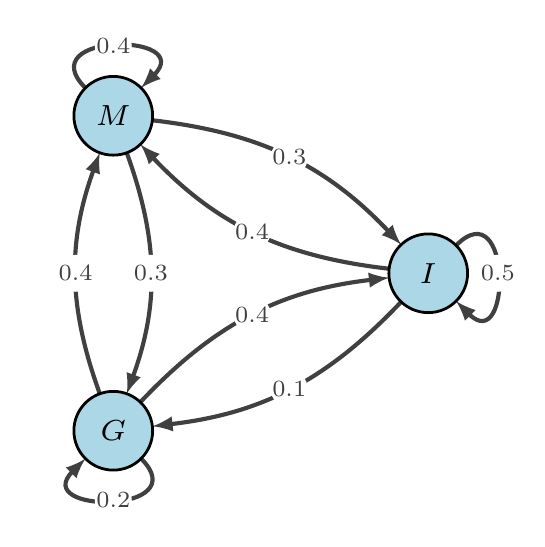
\begin{tikzpicture}
        \drawV{0}{0}{G}
        \drawV{0}{4}{M}
        \drawV{4}{2}{I}
        % Loops
        \drawL{270}{90}{0.2}{G}
        \drawL{90}{90}{0.4}{M}
        \drawL{0}{90}{0.5}{I}
        % Nomal Edges
        \drawE[20]{0.3}{M}{G}
        \drawE[20]{0.4}{G}{M}
        \drawE[20]{0.3}{M}{I}
        \drawE[20]{0.4}{I}{M}
        \drawE[20]{0.1}{I}{G}
        \drawE[20]{0.4}{G}{I}
        
    \end{tikzpicture}
    \caption{Graph of the Network Traffic}
    \label{fig:network-traffic}
\end{figure}
In the graph representation, each node represents a webpage (Google \(G\), Microsoft \(M\), and Intel \(I\)), and the directed edges between them represent the probability of a user moving from one webpage to another. The edge labels indicate these probabilities. This graph can be classified as a directed multigraph because it allows multiple edges between the same pair of nodes (e.g., different probabilities from \(G\) to \(M\) and from \(M\) to \(G\)).

Alternatively, the network can be abstracted as a Finite State Machine (FSM), where each node represents a state corresponding to a webpage, and the directed edges represent the transitions between states with given probabilities. The FSM abstraction emphasizes the state transition process, particularly useful for understanding the dynamic behavior of the system over time.


\subsection*{Finite State Machine Abstraction}
In the FSM abstraction, the network is viewed as a system of states with transitions governed by certain probabilities. Here, each state corresponds to a webpage, and the directed edges (transitions) reflect the probabilities that a user moves from one webpage (state) to another. This abstraction is useful for analyzing the dynamic behavior of the system, such as determining how the state of the system evolves over time and eventually reaches a steady state. This model can help us understand how user distribution across webpages stabilizes and how the system behaves under different initial conditions.

However, this model does not have a clear accept states and input alphabet, I tend to treat it as a directed multigraph.


\subsection*{Graph Abstraction}
In the graph model, we focus on the structure and interconnections of the network. The nodes \(G\), \(M\), and \(I\) represent the different webpages, and the edges represent the possible transitions a user can make from one webpage to another. The probabilities on the edges give us a way to model the likelihood of these transitions. This model is particularly useful for analyzing the overall structure of the network, finding key nodes, and understanding the flow of traffic across the network.


\subsubsection*{Nodes and Edges}
\begin{itemize}
    \item Nodes \(V\): The set of nodes \(V\) represents the different webpages. In this case:
    \[
    V = \{G, M, I\}
    \]
    where \(G\) stands for Google, \(M\) for Microsoft, and \(I\) for Intel.

    \item Edges \(E\): The set of directed edges \(E\) represents the possible transitions between the webpages. Each edge \(e_{ij} \in E\) is associated with a probability \(p_{ij}\) that represents the likelihood of a user transitioning from webpage \(i\) to webpage \(j\). For example:
    \[
    e_{GM} \text{ with probability } p_{GM} = 0.4
    \]
    indicates a 40% probability that a user moves from Google (\(G\)) to Microsoft (\(M\)).
\end{itemize}

\subsubsection*{Adjacency Matrix}
The adjacency matrix \(A\) is a square matrix used to represent the directed multigraph, where each element \(a_{ij}\) indicates the probability of a transition from node \(i\) to node \(j\):
\[
A = 
\begin{bmatrix}
a_{GG} & a_{GI} & a_{GM} \\
a_{IG} & a_{II} & a_{IM} \\
a_{MG} & a_{MI} & a_{MM}
\end{bmatrix}
\]
For the given graph, the adjacency matrix is:
\begin{equation}\label{W4adjmat}
A = \begin{bmatrix}
0.2 & 0.4 & 0.4 \\
0.1 & 0.5 & 0.4 \\
0.3 & 0.3 & 0.4
\end{bmatrix}
\end{equation}


Here, \(a_{ij}\) represents the transition probability from node \(i\) to node \(j\).

\subsubsection*{Degree of Nodes}
The degree of a node in a directed graph can be divided into in-degree and out-degree:
\begin{itemize}
    \item In-degree \(d_{in}(v)\): The in-degree of a node \(v\) is the sum of the probabilities of all edges directed towards that node. For example, the in-degree of node \(M\) is:
    \[
    d_{in}(M) = p_{GM} + p_{IM} + p_{MM} = 0.4 + 0.4 + 0.4 = 1.2
    \]
    \item Out-degree \(d_{out}(v)\): The out-degree of a node \(v\) is the sum of the probabilities of all edges directed away from that node. For example, the out-degree of node \(G\) is:
    \[
    d_{out}(G) = p_{GG} + p_{GM} + p_{GI} = 0.2 + 0.4 + 0.4 = 1.0
    \]
\end{itemize}

\subsubsection*{Weight of Edges}
The weight of an edge $e_{ij} \in E$ is the probability that an object move from state $j$ to $i$, where $i,j\in V$. This is denoted by $w(e_{ij})$.

For example, a user could follow the path \(G \to M\), with the probability of this path being the weight of the edge :
\[
p_{\text{path}} = p(w_{GM})
\]
\
\section*{Problem 1}
\begin{solution}
We use the following expression to show the number of people browsing a webpage $v \in V$.
\[
v_{n} = \sum_{e_{ij}\in E_{in}(v)}( p_{ij}\times i_{n-1})
\]
Where
\begin{itemize}
    \item $v_n$ is the number of people staying at webpage $v$ after $n$ hour, $n\in \Z_{\geq 1}$
    \item $e_{ij}$ is the edge connects from $i$ to $j$, where $i,j\in V$.
    \item $E_{in}(v)$ is the set of edges that goes into node $v$.
    \item $p_{ij}$ is the weight or probability for an user moving from node $i$ to node $j$, which is also $p(e_{ij})$.
\end{itemize}
From what are given, we have
\[
\begin{cases}
    G_0 = 1000\\
    I_0 = 1000\\
    M_0 = 1000
\end{cases}
\]

With these, we have

\begin{align*}
G_1 & =0.2\times 1000+0.1\times 1000+0.3\times 1000 = 600\\
I_1 & =0.5\times 1000+0.4\times 1000+0.3\times 1000 = 1200\\
M_1 & =0.4\times 1000+0.4\times 1000+0.4\times 1000 = 1200
\end{align*}

Therefore, after one hour there will be 600 people on Google's page, 1200 respectively in Microsoft and Intel's page.

\begin{remark}
A interesting finding here is that we can actually get this straight away using the adjacency matrix, but not really the matrix we defined as in (\ref{W4adjmat}).

We construct the adjacency matrix with each row vector representing the possibility of leaving from one node to other nodes (including form a loop), where all elements are the possibility of leaving $G$ to some other nodes including itself, in the next hour. Moreover, we notice that each column of the adjacency matrix are showing the possibility of going into a node from other nodes (including the node it self).

With this notion, we can construct a quite helpful matrix to solve this problem, which is exactly $A^T$, where
\begin{equation}\label{W4adjT}
A^T = 
\begin{bmatrix}
a_{GG} & a_{IG} & a_{MG} \\
a_{GI} & a_{II} & a_{MI} \\
a_{GM} & a_{IM} & a_{MM}
\end{bmatrix}
=
\left[\begin{array}{lll}
0.2 & 0.1 & 0.3 \\
0.4 & 0.5 & 0.3 \\
0.4 & 0.4 & 0.4
\end{array}\right].
\end{equation}

This \textbf{really} inspired me in some of the notions in matrix properties and Graph theory, and I see very strong connections. Transposing the adjacency matrix can be treated as constructing a \textbf{new isomorphic graph} that simply changes the position of each vertices, and has the same connectivity and weights between corresponding nodes. We can show this forms a bijection between the graph of $A$ and $A^T$.

This reminds me that some of the properties of determinants, like interchanging rows or columns and transposing a matrix do not change the determinant, and indeed, isomorphic graphs' adjacency matrices always have equal determinant despite that they are different matrices (All those operations are equivalent to constructing a new isomorphic graph). Another reason that these property hold is that there is a bijective relation between graph and matrix, i.e., for every graph, there is a unique matrix representation. 

Formally, we use class under NBG set theory for prudence (since the 'set' we will define is too general, and can only be proper set, or we call class, in NBG system), and let \( \mathcal{G} \) be the class of all graphs, and \( \mathcal{M} \) be the class of all square matrices with real entries.

Define \( f: \mathcal{G} \rightarrow \mathcal{M} \) as follows:

\[
f(G) = A \text{ where } A \text{ is the adjacency matrix of } G.
\]

The adjacency matrix \( A \) is defined by:

\[
A_{ij} = \begin{cases}
    w(i,j) & \text{if there is an edge between vertices } i \text{ and } j \text{ in } G, \\
    0 & \text{otherwise},
\end{cases}
\]

where \( w(i,j) \) represents the weight of the edge between \( i \) and \( j \).

This function \( f \) is a bijection because:

\begin{itemize}
    \item Every graph has a unique adjacency matrix that encodes its structure and edge weights (If it's a simple graph, we take all weights as 1).
    \item Every matrix in \( \mathcal{M} \) uniquely represents a graph, with the matrix entries corresponding to edge weights (which may be negative, zero, or positive).
\end{itemize}



By transposing the adjacency matrix \( A \), we construct a new matrix \( A^T \) that represents a graph that is isomorphic to the original graph. Formally, if \( A \) represents the adjacency matrix of graph \( G \), then \( A^T \) represents the adjacency matrix of a new graph \( G^T \), where \( G^T \) is an isomorphic graph to \( G \) under the bijection:

\[
f: V(G) \rightarrow V(G^T), \quad \text{where} \quad f(v) = v \text{ for all } v \in V(G)
\]

and for any \( u, v \in V(G) \),

\[
(u, v) \in E(G) \iff (v, u) \in E(G^T).
\]

This bijection preserves the structure of the graph while retains the direction of all edges, effectively allowing us to analyze the incoming traffic to each node (webpage) by considering the transposed adjacency matrix.

The transposed matrix can be used directly to left multiply some column vector of the initial number of people in the corresponding webpage (just like what we will do in problem 2), in this case, we can use 
$\mathbf{x} = 
\begin{bmatrix}
    G_0 \\
    I_0 \\
     M_0\\
\end{bmatrix}
=
\begin{bmatrix}
    1000 \\
    1000 \\
    1000 \\
\end{bmatrix}
$,
and we will have 
\[
A^T \mathbf{x} = \begin{bmatrix}
    0.2\times 1000+0.1\times 1000+0.3\times 1000\\
    0.4\times 1000+0.5\times 1000+0.3\times 1000\\
    1000+0.4\times 1000+0.4\times 1000 +0.4 \times 1000
\end{bmatrix}
=
\begin{bmatrix}
    600\\
    1200\\
    1200
\end{bmatrix}.
\]

This is exactly the same answer, but derived in a different way.

\end{remark}

\end{solution}

\section*{Problem 2}
\begin{solution}
We have derived the transition matrix $\mathbf{A}$ in (\ref{W4adjT}), which is
$
\left[\begin{array}{lll}
0.2 & 0.1 & 0.3 \\
0.4 & 0.5 & 0.3 \\
0.4 & 0.4 & 0.4
\end{array}\right]
$,
by transposing the adjacency matrix of the graph. However, this can also be obtained by just examining the flow of user from the information given.
So we have 

$$\mathbf{A}=
\left[\begin{array}{lll}
0.2 & 0.1 & 0.3 \\
0.4 & 0.5 & 0.3 \\
0.4 & 0.4 & 0.4
\end{array}\right].$$


This allows us to generalise our finding in last problem to the following state transition equation.
\begin{equation}\label{W4state}
\mathbf{x}_n = \mathbf{A} \mathbf{x}_{n-1}, \text{ where } n\in \Z_{\geq 1}, 
\mathbf{x}_n =
\begin{bmatrix}
    G_n & M_n & I_n
\end{bmatrix}^T.
\end{equation}
\end{solution}

\section*{Problem 3}
\begin{solution}
We first provide an alternative way to evaluate the value of $\mathbf{x}_n$ using mathematical induction. The recursive nature of the state transition equation allows us to prove this more easily.

\begin{proof}
    Let the predicate \( P(n) \) be defined as:
    \[
    P(n):\ \mathbf{x}_n = \mathbf{A}^n \mathbf{x}_0
    \]
    We will prove by mathematical induction that \( P(n) \) is true for all \( n \in \mathbb{Z}_{\geq 1} \).

    \textbf{Base Case}

    First, we check the base case where \( n = 1 \). According to the state transition equation, we have \( \mathbf{x}_1 = \mathbf{A} \mathbf{x}_0 \), where \( \mathbf{x}_0 = \begin{bmatrix}1000 \\ 1000 \\ 1000\end{bmatrix} \). Thus:
    \[
    P(1):\ \mathbf{x}_1 = \mathbf{A}^1 \mathbf{x}_0 = \mathbf{A} \mathbf{x}_0
    \]
    Hence, the base case holds.

    \textbf{Inductive Hypothesis}
    
    Assume that \( P(k) \) is true for some arbitrary \( k \geq 1 \). That is, assume:
    \[
    P(k):\ \mathbf{x}_k = \mathbf{A}^k \mathbf{x}_0
    \]

    \textbf{Inductive Step}
    
    We now need to prove that \( P(k+1) \) also holds, i.e., \( \mathbf{x}_{k+1} = \mathbf{A}^{k+1} \mathbf{x}_0 \).

    By the recursive definition of the state transition, we know:
    \[
    \mathbf{x}_{k+1} = \mathbf{A} \mathbf{x}_k
    \]
    Using the inductive hypothesis \( P(k) \), we substitute \( \mathbf{x}_k = \mathbf{A}^k \mathbf{x}_0 \) into the equation:
    \[
    \mathbf{x}_{k+1} = \mathbf{A} \mathbf{x}_k = \mathbf{A} (\mathbf{A}^k \mathbf{x}_0) = \mathbf{A}^{k+1} \mathbf{x}_0
    \]
    Therefore, \( P(k+1) \) holds true.

    Since both the base case and the inductive step have been verified, by the principle of mathematical induction, \( P(n) \) is true for all \( n \geq 1 \).
\end{proof}

Using this result and confirmed by CAS, we have:
\[
\mathbf{x}_3 = 
\mathbf{A}^3 \mathbf{x}_0 =  
\begin{bmatrix}
600 \\
1200 \\
1200
\end{bmatrix}
\]

and 

\[
\mathbf{x}_{24} =
\mathbf{A}^{24} \mathbf{x}_0 =  
\begin{bmatrix}
600 \\
1200 \\
1200
\end{bmatrix}
\]

after rounding.

\begin{remark}
    Numerically, $\mathbf{x}_3$ and $\mathbf{x}_{24}$ can be treated as the same vector. However, they are not exactly identical due to rounding.
\end{remark}    
\end{solution}


\section*{Problem 4}
\begin{solution}
Now we need to calculate $\mathbf{x}_3$ and $\mathbf{x}_{24}$ again with the new initial status $\mathbf{x}_0=[2000,500,500]^T$.

After rounding, we still have 
\[
\mathbf{x}_3 = 
\mathbf{A}^3 \mathbf{x}_0 =  
\left[
\begin{array}{ccc}
600\\
1200\\
1200\\
\end{array}
\right]
\]

and 

\[
\mathbf{x}_{24} =
\mathbf{A}^{24} \mathbf{x}_0 =  
\left[
\begin{array}{ccc}
600\\
1200\\
1200\\
\end{array}
\right]
\].

\begin{remark}
We obtain the final state after changing the initial state because the system's dynamics are unchanged; that is, the process operates within the same graph, and the adjacency matrix (or transition matrix) remains constant. As the system is closed, any non-zero input will converge to a common final state after a sufficient number of iterations.

This situation is reminiscent of the chemical equilibrium system I learned about in high school. Both systems share a similar nature: as long as the initial state is non-zero, the final state of the closed system is determined solely by the transition matrix. After consulting some sources, I realised this is indeed an eigenvalue/eigenvector problem.

Another way to explain this is by considering the properties of the transition matrix, which corresponds to the adjacency matrix of the isomorphic graph.

In graph theory, the power of the adjacency matrix can be very useful for counting the number of possible walks from one vertex to another. The element $\mathbf{A}_{ij}^n$, where $i,j \in V$ and $n \in \mathbb{Z}_{\geq 1}$, represents the number of possible walks of length $n$ from vertex $i$ to vertex $j$ in a simple graph. In the context of a directed multigraph, the meaning of the entries in the adjacency matrix power varies as the weights are defined differently. Here, it can be interpreted as the probability of transitioning to state $j$ from state $i$ after $n$ transitions. When $n \to \infty$, the matrix power will converge, and each part of the system will stabilize, meaning that there will theoretically be no net inflow or outflow from any vertex or state. Since $n$ represents the number of time steps passed, as $n \to \infty$, we obtain a transition matrix that can be used to measure the probability of transitioning from one state to another at any time. This is precisely steady state in a Markov process.
\end{remark}
\end{solution}

\section*{Problem 5}
\begin{solution}
Given that the number of visitors stabilizes to a time-independent constant vector \( \mathbf{x} = [G,I,M]^T \), we will prove that \( \mathbf{x} \) is an eigenvector of the matrix \( \mathbf{A} \) corresponding to the eigenvalue \( \lambda = 1 \).

When the number of visitors stabilizes, it implies that for any further update of the system, the following condition holds:
\[
\mathbf{A}\mathbf{x} = \mathbf{x}.
\]
This equation can be rewritten as:
\[
\mathbf{A}\mathbf{x} = 1 \cdot \mathbf{x}.
\]
Thus, \( \mathbf{x} \) satisfies the equation \( \mathbf{A}\mathbf{x} = \lambda \mathbf{x} \) with \( \lambda = 1 \). Therefore, \( \mathbf{x} \) is an eigenvector of the matrix \( \mathbf{A} \) corresponding to the eigenvalue \( \lambda = 1 \).

In other words, \( \mathbf{x} \) satisfies:
\[
(\mathbf{A} - \mathbf{I})\mathbf{x} = 0,
\]
where \( \mathbf{I} \) is the identity matrix. This confirms that \( \mathbf{x} \) is indeed an eigenvector of \( \mathbf{A} \) associated with the eigenvalue \( \lambda = 1 \).
\end{solution}

\section*{Problem 6}
$$\mathbf{A} = 
\begin{bmatrix}
0.2 & 0.3 & 0.1 \\
0.4 & 0.5 & 0.3 \\
0.4 & 0.4 & 0.4
\end{bmatrix}
$$

When \(\mathbf{A}\) has an eigenvector \(\mathbf{x}\), it satisfies
$$\mathbf{A}\mathbf{x} = \lambda \mathbf{x}.$$
Left multiplying by the identity matrix \(\mathbf{I}\), we have
\[
\mathbf{I}\mathbf{A}\mathbf{x} = \lambda \mathbf{I}\mathbf{x},
\]
and
\[
\mathbf{A}\mathbf{x} - \lambda \mathbf{I}\mathbf{x} = \mathbf{0}.
\]
By the distributive property of matrix multiplication:
\[
(\mathbf{A} - \lambda \mathbf{I})\mathbf{x} = \mathbf{0}.
\]

Note that the eigenvector cannot be \(\mathbf{0}\) as per our assumption. As:
\[
\mathbf{x} = \mathbf{0} \iff \exists (\mathbf{A} - \lambda \mathbf{I})^{-1},
\]
\(\mathbf{A} - \lambda \mathbf{I}\) must be singular (non-invertible).

That is:
\[
|\mathbf{A} - \lambda \mathbf{I}| = 0.
\]

\[
\mathbf{A} - \lambda \mathbf{I} = 
\begin{bmatrix}
 0.2 - \lambda & 0.3 & 0.1 \\
 0.4 & 0.5 - \lambda & 0.3 \\
 0.4 & 0.4 & 0.4 - \lambda \\
\end{bmatrix}
\]

$$\begin{aligned}
\det(\mathbf{A} - \lambda \mathbf{I}) &= 
\begin{vmatrix}
 0.2 - \lambda & 0.3 & 0.1 \\
 0.4 & 0.5 - \lambda & 0.3 \\
 0.4 & 0.4 & 0.4 - \lambda \\
\end{vmatrix}\\
&= (0.2 - \lambda)\begin{vmatrix}
    0.4 - \lambda & 0.4 \\
    0.4 & 0.4 - \lambda
\end{vmatrix}
-0.3 \begin{vmatrix}
    0.4 & 0.3 \\
    0.4 & 0.4 - \lambda
\end{vmatrix}
+ 0.1 \begin{vmatrix}
    0.4 & 0.5 - \lambda \\
    0.4 & 0.4
\end{vmatrix}\\
&= -\lambda^3 + 1.1\lambda^2 - 0.1\lambda = 0
\end{aligned}$$

Factorising this, we have:
\[
-\lambda(\lambda^2 - 1.1\lambda + 0.1) = -\lambda(\lambda - 1)(\lambda - 0.1) = 0
\]

So \(\lambda = 0 \lor \lambda = 1 \lor \lambda = 0.1\).


\section*{Problem 7}
\begin{solution}
To find the eigenvectors, we need to solve
\[
(\mathbf{A} - \lambda \mathbf{I})\mathbf{x} = \mathbf{0}.
\]

When $\lambda = 0$,
$$
\left[\begin{array}{ccc}
0.2 & 0.3 & 0.1 \\
0.4 & 0.5 & 0.3 \\
0.4 & 0.4 & 0.4
\end{array}\right]\left[\begin{array}{l}
x_1 \\
x_2 \\
x_3
\end{array}\right]=\left[\begin{array}{l}
0 \\
0 \\
0
\end{array}\right]
$$

After Elimination we have the RREF

\[
\left[\begin{array}{ccc|c}
1 & 1 & 1 & 0 \\
0 & 1 & -1& 0\\
0 & 0 & 0 & 0
\end{array}
\right]
\]
We introduce a parameter $t$ such that $x_3 = t$.
The solution is 
$\begin{cases}
x_1 = -2t\\
x_2 = t\\
x_3 = t
\end{cases}$.

Let $t = 1$, we have an eigenvector $(-2, 1, 1)$.

%%%

When $\lambda = 1$,
$$
\left[\begin{array}{ccc}
-0.8 & 0.3 & 0.1 \\
0.4 & -0.5 & 0.3 \\
0.4 & 0.4 & -0.6
\end{array}\right]\left[\begin{array}{l}
x_1 \\
x_2 \\
x_3
\end{array}\right]=\left[\begin{array}{l}
0 \\
0 \\
0
\end{array}\right]
$$

After Elimination we have the RREF

\[
\left[\begin{array}{ccc|c}
1 & 1 & -1.5 & 0 \\
0 & 1 & -1& 0\\
0 & 0 & 0 & 0
\end{array}
\right]
\]
We introduce a parameter $t$ such that $x_3 = t$.
The solution is 
$\begin{cases}
x_1 = 0.5t\\
x_2 = t\\
x_3 = t
\end{cases}$.

Let $t = 2$, we have an eigenvector $(1, 2, 2)$.

%%%

When $\lambda = 0.1$,
$$
\left[\begin{array}{ccc}
0.1 & 0.3 & 0.1 \\
0.4 & 0.4 & 0.3 \\
0.4 & 0.4 & 0.3
\end{array}\right]\left[\begin{array}{l}
x_1 \\
x_2 \\
x_3
\end{array}\right]=\left[\begin{array}{l}
0 \\
0 \\
0
\end{array}\right]
$$

Similarly, we have $(-1, 1, 0)$ as our eigenvector.

To sum up, we have eigenvectors
\[
\begin{cases}
    (-1, 1, 0)& \text{when }\lambda = 0.1\\
    (1, 2, 2)& \text{when }\lambda = 1\\
    (-2, 1, 1)& \text{when }\lambda = 0
\end{cases}
\]
\end{solution}


\section*{Problem 8}
\begin{solution}
    
We use the eigenvalues and eigenvectors to construct $\mathbf{D}$ and $\mathbf{V}$.

We have
$$
\mathbf{D} = 
\begin{bmatrix}
    0 & 0 & 0\\
    0 & 1 & 0\\
    0 & 0 & 0.1
\end{bmatrix}
$$
and
$$
\mathbf{V} = 
\begin{bmatrix}
    -2 & 1 & -1\\
    1 & 2 & 1\\
    1 & 2 & 0
\end{bmatrix}
$$
By placing each eigenvector in the column where the corresponding eigenvalue are placed in the diagonal matrix.

We need $\det(\mathbf{V})$  and $\adj(\mathbf{V})$ to get $\mathbf{V}^{-1}$.
$$
\det (V) = -2
\begin{vmatrix}
    2 & 1\\
    2 & 0
\end{vmatrix}
-
\begin{vmatrix}
    1 & 1\\
    1 & 0
\end{vmatrix}
-
\begin{vmatrix}
    1 & 2\\
    1 & 2
\end{vmatrix}
=4+1-0=5
$$
\[
\adj(\mathbf{V}) = (\text{cof}(\mathbf{V}))^T =
\begin{bmatrix}
\begin{vmatrix}2 & 1\\2 & 0\end{vmatrix} & -\begin{vmatrix}1 & 1\\1 & 0\end{vmatrix} & \begin{vmatrix}1 & 2\\1 & 2\end{vmatrix}\\\\
-\begin{vmatrix}1 & -1\\2 & 0\end{vmatrix} & \begin{vmatrix}-2 & -1\\1 & 0\end{vmatrix} &-\begin{vmatrix}-2 & 1\\1 & 2\end{vmatrix}\\\\
\begin{vmatrix}1 & -1\\2 & 1\end{vmatrix}& -\begin{vmatrix}-2 & -1\\1 & 1\end{vmatrix}&
\begin{vmatrix}-2 & 1\\1 & 2\end{vmatrix}
\end{bmatrix}^T
=
\left[\begin{array}{ccc}
-2 & -2 & 3 \\
1 & 1 & 1 \\
0 & 5 & -5
\end{array}\right]
\]

We have
\[
\mathbf{V}^{-1} = \frac{\adj(\mathbf{V})}{\det(\mathbf{V})}
=
\left[\begin{array}{ccc}
-\frac{2}{5} & -\frac{2}{5} & \frac{3}{5} \\
\frac{1}{5} & \frac{1}{5} & \frac{1}{5} \\
0 & 1 & -1
\end{array}\right].
\]

Hence,
\[
\mathbf{A} = 
\mathbf{V}\mathbf{D}\mathbf{V}^{-1}
=
\begin{bmatrix}
    -2 & 1 & -1\\
    1 & 2 & 1\\
    1 & 2 & 0
\end{bmatrix}
\begin{bmatrix}
    0 & 0 & 0\\
    0 & 1 & 0\\
    0 & 0 & 0.1
\end{bmatrix}
\left[\begin{array}{ccc}
-\frac{2}{5} & -\frac{2}{5} & \frac{3}{5} \\
\frac{1}{5} & \frac{1}{5} & \frac{1}{5} \\
0 & 1 & -1
\end{array}\right].
\]
\end{solution}


\section*{Problem 9}

\begin{proof}
We will prove the statement that \(\mathbf{A}^n = \mathbf{V} \mathbf{D}^n \mathbf{V}^{-1}\) for all non-negative integers \(n\) by mathematical induction.

\textbf{Base Case:} For \(n = 0\), we need to verify that:
\[
\mathbf{A}^0 = \mathbf{V} \mathbf{D}^0 \mathbf{V}^{-1}.
\]
Since \(\mathbf{A}^0\) and \(\mathbf{D}^0\) are both identity matrices, we have:
\[
\mathbf{A}^0 = \mathbf{I} = \mathbf{V} \mathbf{I} \mathbf{V}^{-1} = \mathbf{V} \mathbf{V}^{-1} = \mathbf{I}.
\]
This shows that \(\mathbf{A}^0 = \mathbf{V} \mathbf{D}^0 \mathbf{V}^{-1}\) holds true for \(n = 0\).

\textbf{Inductive Step:} Assume that the statement holds for \(n = k\), i.e.,
\[
\mathbf{A}^k = \mathbf{V} \mathbf{D}^k \mathbf{V}^{-1}.
\]
We need to show that it also holds for \(n = k+1\).

Consider:
\[
\mathbf{A}^{k+1} = \mathbf{A}^k \mathbf{A}.
\]
Using the inductive hypothesis, we substitute \(\mathbf{A}^k\) with \(\mathbf{V} \mathbf{D}^k \mathbf{V}^{-1}\):
\[
\mathbf{A}^{k+1} = (\mathbf{V} \mathbf{D}^k \mathbf{V}^{-1}) \mathbf{A}.
\]
Now substitute \(\mathbf{A} = \mathbf{V} \mathbf{D} \mathbf{V}^{-1}\) into the equation:
\[
\mathbf{A}^{k+1} = \mathbf{V} \mathbf{D}^k \mathbf{V}^{-1} \mathbf{V} \mathbf{D} \mathbf{V}^{-1}.
\]
Since \(\mathbf{V}^{-1} \mathbf{V} = \mathbf{I}\), where \(\mathbf{I}\) is the identity matrix, we have:
\[
\mathbf{A}^{k+1} = \mathbf{V} \mathbf{D}^k \mathbf{I} \mathbf{D} \mathbf{V}^{-1} = \mathbf{V} \mathbf{D}^{k+1} \mathbf{V}^{-1}.
\]
Thus, the statement is true for \(n = k+1\).

By the principle of mathematical induction, the statement \(\mathbf{A}^n = \mathbf{V} \mathbf{D}^n \mathbf{V}^{-1}\) holds for all \(n \in \mathbb{N}_0\).
\end{proof}

\section*{Problem 10}
\begin{solution}

    $$
    \mathbf{D}^n = 
    \begin{bmatrix}
        0^n & 0 & 0\\
        0 & 1^n & 0\\
        0 & 0 & 0.1^n
    \end{bmatrix}
    $$
    Taking the limit as $n$ approaches infinity, we get:
    $$
    \lim_{n \to \infty} \mathbf{D}^n = 
    \begin{bmatrix}
        0 & 0 & 0\\
        0 & 1 & 0\\
        0 & 0 & 0
    \end{bmatrix}.
    $$

    With $\mathbf{D}^n$, we can approximate the states of the system over a long period, or at any moment. By what we just obtained and the transition equation (\ref{W4state}), we have stabilised equation for the system, when $n\to \infty$
    \begin{align*}
    \mathbf{x}_n &= \mathbf{A}^n \mathbf{x}_n = \mathbf{V} \mathbf{D}^n \mathbf{V}^{-1} \mathbf{x}_n \\
    &=\left[\begin{array}{ccc}
-2 & 1 & -1 \\
1 & 2 & 1 \\
1 & 2 & 0
\end{array}\right]
\left[\begin{array}{ccc}
0 & 0 & 0 \\
0 & 1 & 0 \\
0 & 0 & 0
\end{array}\right]\left[\begin{array}{ccc}
-\frac{2}{5} & -\frac{2}{5} & \frac{3}{5} \\
\frac{1}{5} & \frac{1}{5} & \frac{1}{5} \\
0 & 1 & -1
\end{array}\right]
\begin{bmatrix}
    G_n\\I_n\\M_n
\end{bmatrix}  \\
&=\left[\begin{array}{ccc}
0 & 1 & 0 \\
0 & 2 & 0 \\
0 & 2 & 0
\end{array}\right]\left[\begin{array}{ccc}
-\frac{2}{5} & -\frac{2}{5} & \frac{3}{5} \\
\frac{1}{5} & \frac{1}{5} & \frac{1}{5} \\
0 & 1 & -1
\end{array}\right]
\begin{bmatrix}
    G_n\\I_n\\M_n
\end{bmatrix} \\
&=\begin{bmatrix}
\frac{1}{5} & \frac{1}{5} & \frac{1}{5} \\
\frac{2}{5} & \frac{2}{5} & \frac{2}{5} \\
\frac{2}{5} & \frac{2}{5} & \frac{2}{5}
\end{bmatrix}
\begin{bmatrix}
    G_n\\I_n\\M_n
\end{bmatrix}
=
\begin{bmatrix}
    \frac{1}{5}(G_n+I_n+M_n)\\\frac{2}{5}(G_n+I_n+M_n)\\\frac{2}{5}(G_n+I_n+M_n)
\end{bmatrix}.
    \end{align*}

As we inferenced earlier, in this condition, we must have 
\[
\begin{bmatrix}
    \frac{1}{5}(G_n+I_n+M_n)\\\frac{2}{5}(G_n+I_n+M_n)\\\frac{2}{5}(G_n+I_n+M_n)
\end{bmatrix}
=
\begin{bmatrix}
   600\\1200\\1200
\end{bmatrix},
\]
as the system is closed, the total number of users is unchanged, still 3000.
\end{solution}

\begin{remark}
    This system is a Markov Chain, which can be analyzed using the properties of Markov processes \parencite{ross_first_2019}. The idea and approach are quite similar, but we can get another perspective of the system's final status. Analyzing the system with Markov Process allows us to find the possibility of users staying in each website (though we have just got the equivalent solution of number of users, and it can be converted to possibility after divided by the total of users).
\begin{definition}[Markov Chain]
 A Markov Chain is a discrete-time stochastic process that exhibits the "memoryless" property, meaning the future state depends only on the present state, not on the sequence of events that preceded it. Formally, if a stochastic process \(\{X_t\}\) satisfies:
    \[
    \Pr(X_{t+1} = s_j \mid X_t = s_i, X_{t-1} = s_{i_{t-1}}, \dots, X_0 = s_{i_0}) = \Pr(X_{t+1} = s_j \mid X_t = s_i),
    \]
    then the process is a Markov Chain.
\end{definition}

    The transition probabilities between states are represented by a transition matrix \( P \), where \( P_{ij} \) denotes the probability of transitioning from state \( s_i \) to state \( s_j \). The matrix \( P \) must satisfy the following properties:
    \begin{itemize}
        \item The sum of the elements in each row is 1.
        \item All elements are non-negative, i.e., \( P_{ij} \geq 0 \).
    \end{itemize}

    A key theorem in Markov Chains is the steady-state distribution theorem. For an irreducible and positive recurrent Markov Chain, there exists a unique steady-state distribution \(\pi\) that satisfies (this is exactly the equation we deduced by approximate $n$ to infinity in problem 10):

    \[
    \pi P = \pi,
    \]

    where \(\pi\) is a row vector and the sum of its elements equals 1:

    \[
    \sum_{i} \pi_i = 1.
    \]

    To find the steady-state distribution, we solve the following linear system:

    \[
    \pi_1 P_{11} + \pi_2 P_{21} + \dots + \pi_n P_{n1} = \pi_1,
    \]
    \[
    \pi_1 P_{12} + \pi_2 P_{22} + \dots + \pi_n P_{n2} = \pi_2,
    \]
    \[
    \vdots
    \]
    \[
    \pi_1 P_{1n} + \pi_2 P_{2n} + \dots + \pi_n P_{nn} = \pi_n,
    \]

    or equivalently in matrix form:

    \[
    \pi (\mathbf{P} - \mathbf{I}) = 0,
    \]

    where \( I \) is the identity matrix (We can also see that this is isomorphic or equivalent to the eigenvector problem of a matrix when $\lambda=1$). Since this system is typically underdetermined (fewer independent equations than unknowns), we impose the normalisation condition (derived from normalisation axiom in probability theory):

    \[
    \sum_{i=1}^n \pi_i = 1,
    \]

    to ensure a unique solution. Solving this system gives us the steady-state distribution \(\pi\).

    The steady-state distribution characterises the long-term behaviour of the Markov Chain, indicating that regardless of the initial state, the system will eventually stabilise.

We are given the state transition matrix \( \mathbf{P} \) as:

\[
\mathbf{P} = \begin{bmatrix}
0.2 & 0.1 & 0.3 \\
0.4 & 0.5 & 0.3 \\
0.4 & 0.4 & 0.4
\end{bmatrix}
\]

The steady-state distribution \( \pi = \begin{bmatrix} \pi_1 & \pi_2 & \pi_3 \end{bmatrix} \) satisfies the equation:

\[
\pi \mathbf{P} = \pi \equiv \pi (\mathbf{P} - \mathbf{I})=0
\]

Expanding this equation gives us the following system of linear equations:

\[
\begin{cases}
-0.8\pi_1 + 0.4\pi_2 + 0.4\pi_3 = 0, \\
0.1\pi_1 - 0.5\pi_2 + 0.4\pi_3 = 0, \\
0.3\pi_1 + 0.3\pi_2 - 0.6\pi_3 = 0.
\end{cases}
\]

Additionally, we have the normalisation condition:

\[
\pi_1 + \pi_2 + \pi_3 = 1.
\]

Now, solving this system of equations, we find:

\[
\begin{cases}
\pi_2 = \pi_3, \\
\pi_1 = \frac{1}{2}\pi_2, \\
\pi_1 + \pi_2 + \pi_3 = 1.
\end{cases}
\]

Substituting the first two equations into the normalisation condition:

\[
\frac{1}{2}\pi_2 + \pi_2 + \pi_2 = 1.
\]

Simplifying, we get:

\[
\frac{5}{2}\pi_2 = 1, \quad \text{so} \quad \pi_2 = \frac{2}{5}.
\]

Thus, we have:

\[
\pi_1 = \frac{1}{5}, \quad \pi_3 = \frac{2}{5}.
\]

The steady-state distribution is therefore:

\[
\pi = \begin{bmatrix} \frac{1}{5} & \frac{2}{5} & \frac{2}{5} \end{bmatrix}.
\]

Therefore, in the long run, there will be 20\% of the users in Google's page, and 40\% respectively in Microsoft and Intel's website.

Another interesting fact is that this is exactly what we have done earlier. The only difference here is the constraint, or assumption for the system. Previously, we used the constraint that the total number of users in the system is always 3000, while here, we assume that the sum of probabilities in each state is 1. Additionally, we find that the solution here and the solution we found earlier are actually linearly dependent on the scalar \(G_n + I_n + M_n\).
\end{remark}



\section*{Problem 11}
\begin{solution}
We can visualize the new graph, we still call it $G$ from now on.

\begin{figure}[H]
    \centering
    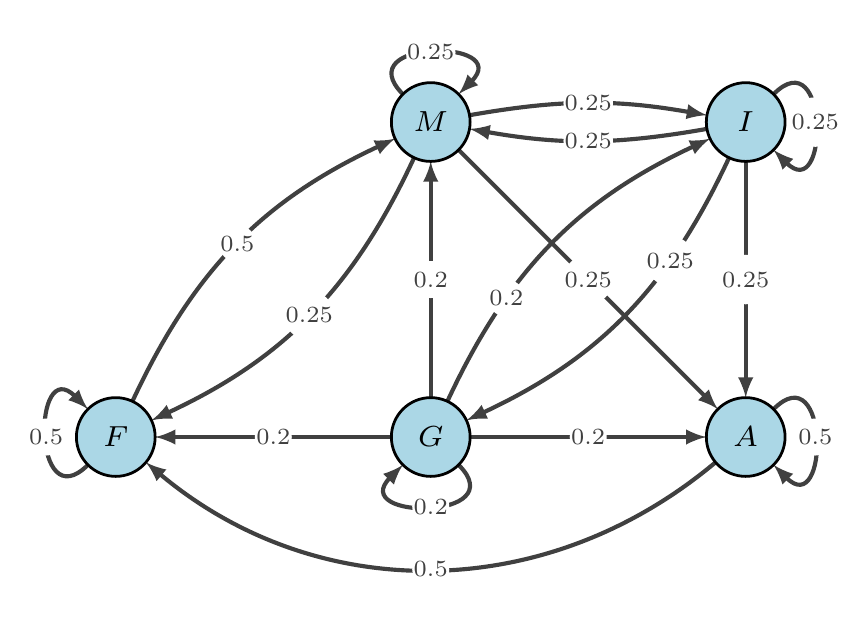
\begin{tikzpicture}
    %Notes
        \drawV{0}{0}{G}
        \drawV{0}{4}{M}
        \drawV{-4}{0}{F}
        \drawV{4}{4}{I}
        \drawV{4}{0}{A}

    % Noemal Edges
        \drawE[10]{0.25}{I}{M}
        
        \drawE[10]{0.25}{M}{I}
        \Edge[Direct, bend = 0, label = 0.25, fontscale = 1.2, distance=0.5](M)(A)
        \drawE{0.25}{I}{A}
        %\drawE[15]{0.25}{I}{G}
        %\drawE[15]{0.2}{G}{I}
        \Edge[Direct, bend = 20, label = 0.2, fontscale = 1.2, distance=0.3](G)(I)
        \Edge[Direct, bend = 20, label = 0.25, fontscale = 1.2, distance=0.3](I)(G)
        \drawE{0.2}{G}{M}
        \drawE{0.2}{G}{A}
        \drawE{0.2}{G}{F}
        \drawE[20]{0.25}{M}{F}
        \drawE[20]{0.5}{F}{M}
        \drawE[40]{0.5}{A}{F}

    % Loops
        \drawL{270}{90}{0.2}{G}
        \drawL{0}{90}{0.25}{I}
        \drawL{180}{90}{0.5}{F}
        \drawL{-270}{90}{0.25}{M}
        \drawL{0}{90}{0.5}{A}
    \end{tikzpicture}
    \caption{Extended Network Traffic}
    \label{fig:enter-label}
\end{figure}
Since
\begin{quote}
\textbf{After each hour, a person visiting a webpage has an equal
chance of staying on the webpage or following any one of its links.}
\end{quote}

We can deduce, as what we have marked in the graph, the adjacency matrix of $G$, where $G_{ij}$ is $w(e_{ij})$, and the subscripts are defined by the lexicographical order of company names, $i, j \in \{1, 2, 3, 4, 5\}$. 
\[
\mathbf{G} = 
\begin{bmatrix}
0.5 & 0 & 0.2 & 0.25 & 0.25 \\
0.5 & 0.5 & 0.2 & 0 & 0.25 \\
0 & 0 & 0.2 & 0.25 & 0 \\
0 & 0 & 0.2 & 0.25 & 0.25 \\
0 & 0.5 & 0.2 & 0.25 & 0.25 \\
\end{bmatrix}
\]

\begin{remark}
This time we do not transpose it, since we rearrange the subscripts in the way that satisfies each row corresponding to walks ending at each node, in alphabetical order. We can write the adjacency matrix in any ways that benefit the problem-solving. 

In $\mathbf{G}$, we always have the sum of any column is 1, this is because
\[
\forall v\in V, d_{out}(v) = \sum_{e\in E_{out}(v)} w(e) = 1.
\]
\end{remark}
\end{solution}

\section*{Problem 12}
\begin{solution}
    Since this is a 5 by 5 matrix, it takes more time to look into its matrix power or diagnolization, instead, we can just treat it as a transition probability matrix for a Markov Chain problem, making it easier to solve (by solving a system of linear equation).

    We suppose that when the system is stable, the steady state is defined by the row vector
    \[
    \pi = \begin{bmatrix}P_A & P_F & P_G & P_I & P_M\end{bmatrix},
    \]
    where each entry is the possibility of an individual in states $v\in V$ (practically, probability of browsing the corresponding webpage).
    \begin{remark}
        This reminds me that it's kind of like random walk problem in graph.
    \end{remark}

    When the system is stable, we have 
    \[
    \pi \mathbf{G} = \pi.
    \]
    Right multiply $\mathbf{I}$, we have
    \[
    \pi (\mathbf{G} - \mathbf{I}) = 0,
    \]
    where
    \[
    \mathbf{G} - \mathbf{I} =
    \begin{bmatrix}
    -0.5 & 0 & 0.2 & 0.25 & 0.25 \\
    0.5 & -0.5 & 0.2 & 0 & 0.25 \\
    0 & 0 & -0.8 & 0.25 & 0 \\
    0 & 0 & 0.2 & -0.75 & 0.25 \\
    0 & 0.5 & 0.2 & 0.25 & -0.75 \\
    \end{bmatrix}
    \]

    Now we only need to solve the system of linear equation to get the steady state of the system.

    We have the augmented matrix 
    $$[\mathbf{G} - \mathbf{I} \mid \0]
    =
    \left[\begin{array}{ccccc|c}
    -0.5 & 0 & 0.2 & 0.25 & 0.25 & 0 \\
    0.5 & -0.5 & 0.2 & 0 & 0.25 & 0 \\
    0 & 0 & -0.8 & 0.25 & 0 & 0 \\
    0 & 0 & 0.2 & -0.75 & 0.25 & 0 \\
    0 & 0.5 & 0.2 & 0.25 & -0.75 & 0
    \end{array}\right].
    $$

    After Gaussian elimination, we have RREF
    $$
    \left[\begin{array}{ccccc|c}
    1 & 0 & 0 & 0 & -\frac{8}{11} & 0 \\
    0 & 1 & 0 & 0 & -\frac{14}{11} & 0 \\
    0 & 0 & 1 & 0 & -\frac{5}{44} & 0 \\
    0 & 0 & 0 & 1 & -\frac{4}{11} & 0 \\
    0 & 0 & 0 & 0 & 0 & 0
    \end{array}\right].
    $$

    Hence,
    \begin{equation}
    \begin{cases}
    P_A=\frac{8}{11} t \\
    P_F=\frac{14}{11} t \\
    P_G=\frac{5}{44} t \\
    P_I=\frac{4}{11} t \\
    P_M=t
    \end{cases}.
    \end{equation}

    \begin{remark}
    Here we can see a very interesting fact, that this system's steady status, is dependable to $P_M$. This is actually not surprising and very easy to explain.
    This is because $M$ is the most significant state in the system, and it has the greatest number of edges among all nodes. Moreover, we can already see the ranking here, as $t>0$.
    \end{remark}
    With the normalisation condition \(P_A + P_F + P_G + P_I + P_M = 1\), we will manage to solve $\pi$.

    We substitute the expressions for \( P_A \), \( P_F \), \( P_G \), \( P_I \), and \( P_M \) into the normalization condition \( P_A + P_F + P_G + P_I + P_M = 1 \):

\[
\frac{8}{11}t + \frac{14}{11}t + \frac{5}{44}t + \frac{4}{11}t + t = 1
\]

To solve for \( t \), first combine the terms:

\[
\left(\frac{8}{11} + \frac{14}{11} + \frac{5}{44} + \frac{4}{11} + 1\right)t = 1
\]

Next, find a common denominator for the fractions and sum them:

\[
\frac{32}{44} + \frac{56}{44} + \frac{5}{44} + \frac{16}{44} + \frac{44}{44} = \frac{153}{44}
\]

So, the equation simplifies to:

\[
\frac{153}{44}t = 1,
\]

and

\[
t = \frac{44}{153}.
\]

Thus, the values of \( P_A \), \( P_F \), \( P_G \), \( P_I \), and \( P_M \) are given by:

\[
\begin{aligned}
    P_A &= \frac{8}{11} \cdot \frac{44}{153} = \frac{32}{153} \\
    P_F &= \frac{14}{11} \cdot \frac{44}{153} = \frac{56}{153} \\
    P_G &= \frac{5}{44} \cdot \frac{44}{153} = \frac{5}{153} \\
    P_I &= \frac{4}{11} \cdot \frac{44}{153} = \frac{16}{153} \\
    P_M &= \frac{44}{153}
\end{aligned}
\]

Finally, we have determined the steady-state distribution \( \pi \):

\[
\pi = \left(\frac{32}{153}, \frac{56}{153}, \frac{5}{153}, \frac{16}{153}, \frac{44}{153}\right)
\]

Therefore, we have 
\[
P_F > P_M > P_A > P_I > P_G,
\]

which means that the ranking (higher to lower) is: Facebook, Microsoft, Apple, Intel, and Google.
\end{solution}


\printbibliography
\end{document}
